\documentclass[a4j,10pt,twocolumn]{utf8/abstract}
%\documentclass[a4j,9pt,twocolumn]{abstract}
\usepackage[dvipdfmx]{graphicx}
\usepackage{amssymb}
\usepackage[varg]{txfonts}
%%% \begin{document}の前に,各エントリーを記述する

\title{mruby Bytecode Loader Using Bluetooth in Multi-VM Environment}	% 論文のタイトル
\author{山本 拓朗} 		% 著者
\studentid{09C12174} 	% 学籍番号
\lab{潮}		% 研究室名

% 英語なら以下2行を定義
\englishtitle
\jptitle{Bluetoothを用いたマルチVM対応mrubyバイトコードローダ}  % 日本語のタイトル
 
\begin{document}
\absttitle 		% 表題の出力

\section{まえがき}
近年,組込みシステムは複雑化・大規模化しているため,組込みソフトウェアの生産性が問題になっている.
組込みソフトウェア開発の生産性の向上を目的として,組込みシステム向けのスクリプト言語であるmruby(軽量Ruby)を適用させたコンポーネントベース開発が可能なフレームワークであるmruby on TECSが提案されている \cite{mrubyontecs}.

現状のmruby on TECSでは,プラットフォームにmrubyバイトコードを組み込んでいるため,mrubyプログラムを修正する度にコンパイル・リンクし直す必要がある.
さらに,マルチVMを提供しているが,複数のmrubyアプリケーションを効率良く並行動作させるには開発者がリアルタイムOSの機能を熟知している必要がある.

本研究では,mruby on TECSの拡張として,mrubyアプリケーションのバイトコードをBluetoothで転送することで開発効率を向上させる.
さらに,複数のmrubyアプリケーションを協調動作できるフレームワークを提案する.

\section{既存フレームワークの問題点}
mruby on TECSは,mrubyと,組込みシステムに適したコンポーネントシステムであるTECS (TOPPERS Embedded Component System) を組み合わせたフレームワークである.

スクリプト言語は生産性が高い反面,C言語に比べると実行速度が遅いため,組込みシステムに適用するのは難しい.
mruby on TECSでは,mrubyプログラムからC言語の関数を呼ぶ機能を提供しており,mrubyに比べて,アプリケーションを約100倍速く実行できる.

mruby on TECSでは,mrubyプログラムを修正する度にターゲットデバイスでSDカードを抜き差しし,OSを再起動する必要がある.
さらに,複数のmrubyアプリケーションを並行実行させる場合,開発者がタスクを待ち状態へ遷移させるOSの機能を呼び出さなければならない.
 
\section{提案フレームワーク}
提案フレームワークは,mruby on TECSを拡張して,Bluetoothを用いたmrubyバイトコードローダと,実用的なマルチタスク処理の実装を行った.
システムモデルを図\ref{fig:system_model}に示す.
\begin{figure}[h]
    \centering
    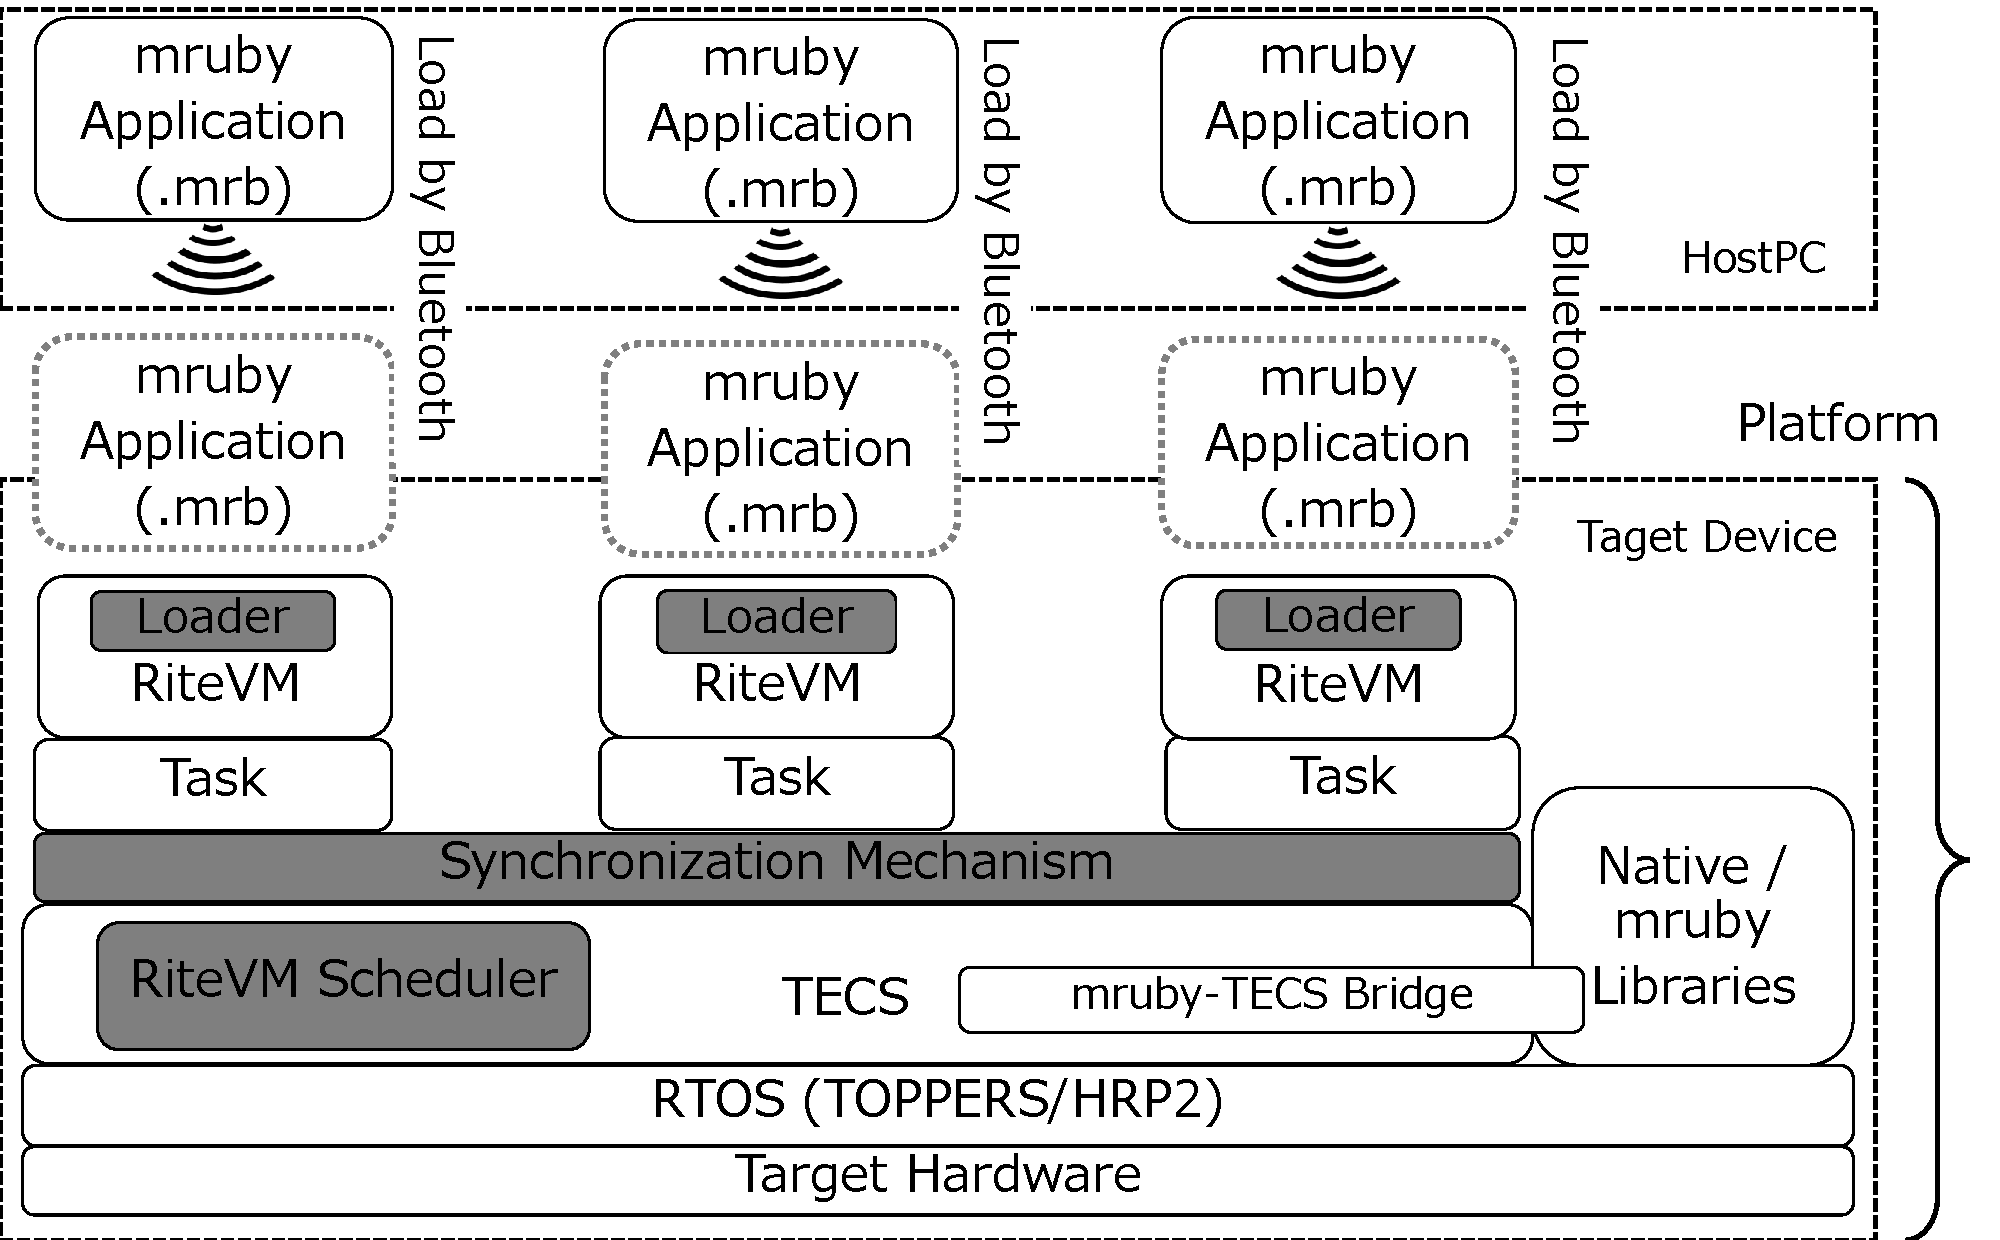
\includegraphics[width=7cm,clip]{Abst_SystemModel.pdf}
    \caption{システムモデル}
    \label{fig:system_model}
\end{figure}

提案フレームワークでは,プラットフォーム(図\ref{fig:system_model}の下部)をコンパイル・リンクし,ターゲットデバイス上で起動する.
ホストPC側では,mrubyアプリケーション (.rb) をバイトコード (.mrb) にコンパイルし,Bluetoothを通してターゲットデバイスにバイトコードを転送する.
ターゲットデバイス側では,RiteVMに実装されたローダが転送されたバイトコードを受信し,すでにプラットフォームに含まれているmrubyライブラリと合わせてアプリケーションを実行する.
これによって,SDカードを抜き差しする手間やOSを再起動する時間が省けるため,作業効率を上げることができる.

さらに,各VMの処理を平等に実行するRiteVMスケジューラを提供することで,マルチタスク処理を効率的に利用できる.
%$\mu$ITRON \cite{microITRON} のサービスコールである{\it rotateReadyQueue}を使った
%開発者にとって使いやすい設計にした.
%{\it rotateReadyQueue}は,同じ優先度のタスクの実行順序を切り替える機能である.
複数タスク間の同期にはイベントフラグ処理を適用し,すべてのタスクが同時に起動するように実装した.
イベントフラグのセットパターンや待ちパターンは,各コンポーネントの属性として定義する.
これによって,VMの数に関わらず,同じCファイルを利用できる.

提案フレームワークでは,RiteVMやRiteVMスケジューラ,イベントフラグはすべてTECSのコンポーネントとして実装されているため,開発者の必要に応じて容易に機能の取り外しができる.

表\ref{tab:comparison}に,提案フレームワークと既存フレームワークの比較を示す.
提案フレームワークでは,Bluetoothを用いたバイトコードローダに加え,VMスケジューラおよびアプリケーションの同期が可能になった.

\section{結論}
Bluetoothを用いたmrubyバイトコードローダによって,mruby on TECSでのソフトウェア開発の作業効率を向上させ,RiteVMスケジューラは複数のmrubyアプリケーションを効率良く実行する.
さらに,提案フレームワークで提供される機能はコンポーネントであるため,機能の取り外しや再利用が容易になる.

実験評価では,ローダによる作業効率の向上やオーバヘッドの少ないマルチタスク設計の有用性,コンポーネントベース開発の利点を示した.

\begin{table}[t]
    \centering
    \caption{関連研究}
    \scriptsize
    {\tabcolsep=0.1cm
    \begin{tabular}{c||c|c|c|c}
        & \shortstack{Bluetooth\\Loader} & \shortstack{VM\\Managenment} & \shortstack{VM\\Scheduler} & \shortstack{Synchronization\\of Application} \\ \hline
        eLua                &            &            & &           \\
        Owl system          &            &            & &           \\
        mruby on TECS       &            & \checkmark & &           \\
        Proposed framework  & \checkmark & \checkmark & \checkmark &\checkmark \\
    \end{tabular}
    }
    \label{tab:comparison}
\end{table}


%\bibliographystyle{junsrt}
%\bibliography{refs}
\begin{thebibliography}{1}
\bibitem{mrubyontecs} T. Azumi, and Y. Nagahara, and H. Oyama, and N. Nishio, 
    ``mruby on TECS: Component-Based Framework for Running Script Program," 
    in Proceedings of the 18th IEEE International Symposium on Real-Time Distributed Computing (ISORC), 
    pp.252-259, 
    2015. 
\end{thebibliography}
\newpage
\pagebreak
\end{document}
